\documentclass[14pt]{beamer} %Makes presentation
%\documentclass[14pt,handout]{beamer} %Makes Handouts
\input{preamble}
\usepackage{tikz}
\usetikzlibrary{shapes,arrows,decorations.pathreplacing}

\title{Practical Issues}

\date[]{}



\begin{document}

\frame{\titlepage}

\frame{\tableofcontents}

\section[]{Administrative Stuff}
\frame{\tableofcontents[currentsection]}

\frame{

\frametitle{Administrative Stuff}

\begin{enumerate}\itemsep1em
\item Summative Essay Deadline
	\begin{itemize}
	\item Tuesday LT Week 1
	\end{itemize}

\item Topics for Weeks 6--11
\end{enumerate}

}


\begin{frame}

\frametitle{Increasing/Decreasing Power}

\begin{columns}
\begin{column}{0.5\textwidth}
\begin{block}{Increases Power}
\begin{itemize}\itemsep1em
\item Bigger sample
\item Precise measures
\item Covariates?
\end{itemize}
\end{block}
\end{column}

\begin{column}{0.5\textwidth}
\begin{block}{Decreases Power}
\begin{itemize}\itemsep1em
\item Attrition
\item Noncompliance
\item Clustering
\end{itemize}
\end{block}
\end{column}
\end{columns}

\end{frame}


\frame{

\frametitle{Covariates in Experiments}

\begin{itemize}\itemsep1em
\item<2-> Identification of a causal effect only requires randomization
\item<2-> We don't need to include covariates in analysis!

	\begin{align}
	Y & = \beta_0 + \beta_1 X + \epsilon \\
	Y & = \beta_0 + \beta_1 X + \beta_{2-J} Z + \epsilon
	\end{align}

\item<4-> Independence of potential outcomes from treatment assignment is an \textit{asymptotic} property of randomization!
\end{itemize}

}

\frame{

\frametitle{Block Randomization I}

\begin{itemize}\itemsep1em
\item<2-> Basic idea: randomization occurs within strata defined \textit{before} treatment assignment
\item<3-> CATE is estimate for each stratum; aggregated to SATE
\item<4-> Why?
	\begin{itemize}
	\item Eliminate chance imbalances
	\item Optimized for estimating CATEs
	\item More precise SATE estimate
	\end{itemize}
\end{itemize}

}

\begin{frame}[fragile]

\begin{center}
\begin{tabular}{lcccccccc}
Exp. & \multicolumn{4}{c}{Control} & \multicolumn{4}{c}{Treatment} \\ \midrule
1 & M & M & M & M & F & F & F & F \\
2 & M & M & M & F & M & F & F & F \\
3 & M & M & F & F & M & M & F & F \\
4 & M & F & F & F & M & M & M & F \\
5 & F & F & F & F & M & M & M & M \\ \bottomrule
\end{tabular}
\end{center}

\end{frame}

\frame{

\begin{center}

\begin{tabular}{rrrr}
Obs. & $X_{1i}$ & $X_{2i}$ & $D_i$ \\ \midrule
1 & Male & Old & 0 \\
2 & Male & Old & 1 \\  \midrule
3 & Male & Young & 1 \\
4 & Male & Young & 0 \\ \midrule
5 & Female & Old & 1 \\
6 & Female & Old & 0 \\ \midrule
7 & Female & Young & 0 \\
8 & Female & Young & 1 \\ \bottomrule
\end{tabular}
\end{center}

}

\frame[label=blocking2]{

\frametitle{Block Randomization II}

\begin{itemize}\itemsep1em
\item Blocking ensures ignorability of all covariates used to construct the blocks
\item Incorporates covariates explicitly into the \textit{design}
\item<2-> When is blocking \textit{statistically} useful?
	\begin{itemize}
	\item<3-> If those covariates affect values of potential outcomes, blocking reduces the variance of the SATE
	\item<4-> Most valuable in small samples
	\item<5-> Not valuable if all blocks have similar potential outcomes
	\end{itemize}
\end{itemize}

}



\frame{

\frametitle{Statistical Properties I}

\small

Complete randomization:\\
$$SATE = \frac{1}{n_1}\sum Y_{1i} - \frac{1}{n_0}\sum Y_{0i}$$

\vspace{2em}

Block randomization:\\
$$SATE_{blocked} = \sum_{1}^{J} \left( \dfrac{n_j}{n} \right)  (\widehat{CATE}_j)$$

}


\frame{

\begin{center}

\begin{tabular}{rrrrrr}
Obs. & $X_{1i}$ & $X_{2i}$ & $D_i$ & $Y_i$ & CATE \\ \midrule
1 & Male & Old & 0 & 5 & \multirow{2}{*}{\onslide<2->{5}} \\
2 & Male & Old & 1 & 10 \\  \midrule
3 & Male & Young & 1 & 4 & \multirow{2}{*}{\onslide<3->{3}} \\
4 & Male & Young & 0 & 1 \\ \midrule
5 & Female & Old & 1 & 6 & \multirow{2}{*}{\onslide<4->{4}} \\
6 & Female & Old & 0 & 2 \\ \midrule
7 & Female & Young & 0 & 6 & \multirow{2}{*}{\onslide<5->{3}} \\
8 & Female & Young & 1 & 9 \\ \bottomrule
\end{tabular}
\end{center}

}

\frame{

\frametitle{SATE Estimation}

\begin{align*}
SATE &= \left(\dfrac{2}{8}*5\right) + \left(\dfrac{2}{8}*3\right) + \left(\dfrac{2}{8}*4\right) + \left(\dfrac{2}{8}*3\right) \\ \vspace{1em}
&= 3.75
\end{align*}

\onslide<2->{The blocked and unblocked estimates are the same here because $Pr(Treatment)$ is constant across blocks and blocks are all the same size.}

}

\frame{

\frametitle{SATE Estimation}

\small

\begin{itemize}
\item We can use weighted regression to estimate this in an OLS framework
\item Weights are the inverse prob. of being treated w/in block
\begin{itemize}
\item Pr(Treated) by block: $p_{ij} = Pr(D_i = 1 | J=j) $
\item Weight (Treated): $ w_{ij} = \dfrac{1}{p_{ij}} $
\item Weight (Control): $ w_{ij} = \dfrac{1}{1-p_{ij}} $
\end{itemize}
\end{itemize}

}


\frame{

\frametitle{Statistical Properties II}

\small

Complete randomization:\\
$$\widehat{SE}_{SATE} = \sqrt{\dfrac{\widehat{Var}(Y_0)}{n_0} + \dfrac{\widehat{Var}(Y_1)}{n_1}}$$

\vspace{1em}

Block randomization:\\
$$\widehat{SE}_{SATE_{blocked}} = \sqrt{\sum_{j=1}^{J} \left( \dfrac{n_j}{n} \right)^2  \widehat{Var}{(CATE_j)}}$$

\only<2->{When is the blocked design more efficient?}

}


\frame{\huge\vskip20pt\textbf{Questions?}}


\frame{

\frametitle{Baseline Outcome Measure}

\begin{itemize}\itemsep0.5em
\item Recall our key definition:
\end{itemize}

	\begin{quote}\small
		The observation of units after, \textbf<2->{and possibly before}, a randomly assigned intervention in a controlled setting, which tests one or more precise causal expectations
	\end{quote}

\begin{itemize}\itemsep0.5em

\item<3-> Pretreatment measures of the outcome can be particularly helpful!

\end{itemize}
}

\frame{

\frametitle{Baseline Outcome Measure}

\begin{itemize}\itemsep0.5em
\item<1-> This changes our estimator of $ATE$ from simple \textit{mean-difference} to \textit{difference-in-differences} (DID)

	\begin{align*}
	(\hat{Y}_{0,t+1} - \hat{Y}_{0,t}) - (\hat{Y}_{j,t+1} - \hat{Y}_{j,t})
	\end{align*}

\item Advantageous because variance for paired samples decreases as correlation between $Y_0$ and $Y_1$ increases
\end{itemize}

}

\frame{
	\begin{center}
	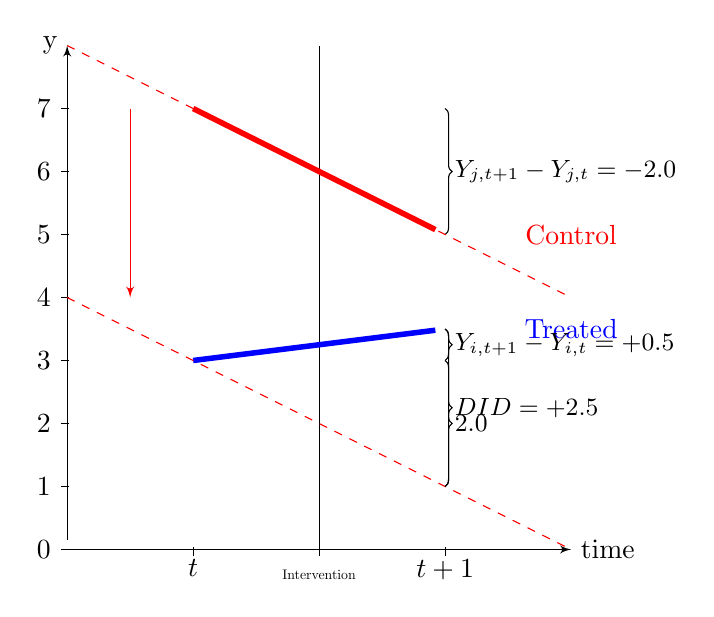
\begin{tikzpicture}[>=latex', scale=0.8]
        \draw[->] (0,0) node (origin) {}  -- (8,0) node[right] (xaxis) {time};
        \draw[->] (origin) -- (0,8) node[left] (yaxis) {y};
        % x ticks
        \foreach \x in {2,4,6}
        	\draw (\x,1pt) -- (\x,-3pt) node[anchor=north] {};
        \draw (2,0) node[below] (before) {$t$};
        \draw (6,0) node[below] (after) {$t+1$};
        \draw (4,-0.25) node[below, scale=0.5] (IV) {Intervention};
        % y ticks
        \foreach \y in {0,...,7}
             \draw (1pt,\y) -- (-3pt,\y) node[anchor=east] {$\y$};
        % intervention
        \draw (4,0) -- (4,8);

        % line
        \draw<2-> (6,3.5) node (tr) {};
        \draw<3-> (6,5) node (ctrl) {};
        \draw<2-3>[blue] (8,3.5) node (trlab) {Treated};
        \draw<3-3>[red] (8,5) node (ctrllab) {Control};        
        \draw<2->[blue, line width=2pt] (2,3) -- (tr);
        \draw<3->[red, line width=2pt] (2,7) -- (ctrl);
        
        % diffs
        \draw<4-6>[right,decorate,decoration={brace,mirror}] 
        	(6,3) -- (6,3.5) node[right, pos=0.5] (idiff) {\small $Y_{i,t+1} - Y_{i,t} = +0.5$};
        \draw<4-6>[right,decorate,decoration={brace}] 
            (6,7) -- (6,5) node[right, pos=0.5] (jdiff) {\small $Y_{j,t+1} - Y_{j,t} = -2.0$};
        
        % trends
        \draw<5-6>[red,->] (1,7) -- (1,4);
        \draw<5->[red, dashed] (0,8) -- (8,4);
        \draw<5->[red, dashed] (0,4) -- (8,0);
        \draw<6>[right,decorate,decoration={brace}] 
            (6,3) -- (6,1) node[right, pos=0.5] (idiff2) {\small $2.0$};
        \draw<7>[right,decorate,decoration={brace}] 
            (6,3.5) -- (6,1) node[right, pos=0.5] (idiff2) {\small $DID = +2.5$};
                        
        
    \end{tikzpicture}
    \end{center}
}


\begin{frame}
\frametitle{Statistical Advantages I}	

In post-treatment-only designs:

\begin{equation*}
\widehat{ATE}_{Diff} = \dfrac{\sum_{i=1}^{n_1} (x_{i,1,t+1})}{n_1} - \dfrac{\sum_{i=1}^{n_0} (x_{i,0,t+1})}{n_0}
\end{equation*}

The variance of this estimate is:

\begin{align*}
Var(\widehat{ATE}_{Diff}) &=  Var(\bar{Y}_{1,t+1}) + Var(\bar{Y}_{0,t+1})%\\
%&= \dfrac{\frac{1}{n_1}\sum_{i=1}^{n_1} (x_{i,1} -\bar{x}_1)^2}{n_1} + \dfrac{\frac{1}{n_0}\sum_{i=1}^{n_0} (x_{i,0} -\bar{x}_1)^2}{n_0}
\end{align*}
\end{frame}

\frame{
\frametitle{Statistical Advantages II}

In pre/post-treatment designs:

\begin{equation*}
\widehat{ATE}_{DID} = \dfrac{\sum_{i=1}^{n_1} (x_{i,1,t+1} - x_{i,1,t})}{n_1} - \dfrac{\sum_{i=1}^{n_0} (x_{i,0,t+1} - x_{i,0,t})}{n_0}
\end{equation*}

The variance of this estimate is:

\small

\begin{align*}
Var(\widehat{ATE}_{DID}) &=  Var(\bar{Y}_{1,t+1} - \bar{Y}_{1,t}) + Var(\bar{Y}_{0,t+1} - \bar{Y}_{0,t}) \\
&= \left(Var(\bar{Y}_{1,t+1}) + Var(\bar{Y}_{1,t}) - Cov(\bar{Y}_{1,t+1}, \bar{Y}_{1,t})\right) \\
&+ \left(Var(\bar{Y}_{0,t+1}) + Var(\bar{Y}_{0,t}) - Cov(\bar{Y}_{0,t+1}, \bar{Y}_{0,t}) \right)
\end{align*}

}



\begin{frame}[fragile]

\small

\begin{verbatim}
# create some fake data
set.seed(54321)
n <- 400L
y0 <- rnorm(n)
x <- rbinom(n, 1L, 0.5)

# high Cor(y0, y1)
y1a <- y0 + 0.25*x + rnorm(n, sd = 0.25)
summary(lm(y1a ~ x))
summary(lm(I(y1a-y0) ~ x))

# low Cor(y0, y1)
y1b <- y0 + 0.25*x + rnorm(n, sd = 2)
summary(lm(y1b ~ x))
summary(lm(I(y1b-y0) ~ x))
\end{verbatim}

\end{frame}



\frame{

\frametitle{Practicalities of blocking}

\begin{itemize}\itemsep1em
\item Blocked randomization and use of pre-treatment measures only works in some circumstances

\item Need to observe covariates pre-treatment in order to block on them

	\begin{itemize}
	\item Challenging in a cross-sectional design
	\end{itemize}

\item The cost of gathering pre-treatment data might also outweigh the gain in precision

	\begin{itemize}
	\item May introduce other biases
	\end{itemize}

\end{itemize}

}


\section{Practical Issues}
\frame{\tableofcontents[currentsection]}



\frame{

\frametitle{Discussion Questions}

\small

\begin{enumerate}
\item How do we know if an experiment worked (well)? What criteria should we apply for evaluating this?
\item What is a failure of randomization? How do we avoid it? When is randomization simple versus difficult?
\item What is noncompliance? Why does it occur? What consequences does it have for experimental inference? 
\item What can we do about noncompliance? Is it a problem that can be solved?
\item Is experimentation ethical? Why or why not?
\end{enumerate}

}


\frame{

\frametitle{Randomization Failure}

\begin{columns}
\begin{column}{.5\textwidth}
\begin{block}{Randomization Failure}

The process of physical randomization was distorted such that assignment was not random.

\end{block}
\end{column}
\begin{column}{.5\textwidth}
\begin{block}{Imbalance}

Physical randomization was used but the treatment groups were not comparable on covariates.

\end{block}
\end{column}
\end{columns}

}


\frame{
\frametitle{Noncompliance}

\begin{itemize}\itemsep1em
\item Compliance is when individuals receive and accept the treatment to which they are assigned
\item Noncompliance:\\{\small ``when subjects who were assigned to receive the treatment go untreated or when subjects assigned to the control group are treated'' \footnote{Gerber \& Green. 2012. \textit{Field Experiments}, p.132.}}
\end{itemize}
}


\frame{

\frametitle{Why do we care?}

\begin{itemize}\itemsep1em
\item<2-> Factors other than randomization explain why individuals receive their treatment
\item<3-> Reduced power
\item<4-> Typically a downwardly biased estimate of SATE
\end{itemize}

}

% noncompliance and intention-to-treat effects

\frame{

\frametitle{Types of noncompliance}

\begin{columns}
\begin{column}{.5\textwidth}
\begin{block}{Asymmetric}

\begin{itemize}
\item Some assignment to treatment A take treatment B instead
\end{itemize}

\vspace{1.2em}

\end{block}
\end{column}
\begin{column}{.5\textwidth}
\begin{block}{Symmetric}

\begin{itemize}
\item Some assignment to treatment A take treatment B instead, and vice versa
\end{itemize}

\end{block}
\end{column}
\end{columns}

}


\frame{

\frametitle{What can we do?}

\begin{itemize}\itemsep1em
\item Intention-to-treatment (ITT) estimation
\item As-treated analysis
\item Something else
\end{itemize}

}

\frame{

\frametitle{Intention-to-treat}

\begin{itemize}\itemsep1em
\item Ignore the treatment actually received
\item Compared units assigned to each treatment condition:\\

$ITT = \overline{Y}_1 - \overline{Y}_0$

\item Tends to underestimate effect of treatment
\end{itemize}

}

\frame{

\frametitle{As-Treated Analysis}

\begin{itemize}\itemsep1em
\item Ignore treatment assignment and analyse as an observational study
\item Moves us out of experimental territory
\item Comparison has no causal interpretation
\end{itemize}

}

\frame{
\frametitle{Something else}

\small

\begin{itemize}\itemsep1em
\item Noncompliance \textit{asymmetric} if only in one group
	
\item We can use a ``Wald estimator'' to estimate the ``local average treatment effect'' (LATE):\\
	$LATE = \dfrac{ITT}{\% Compliant}$

\item Effect is \textit{local} to those whose treatment status could be manipulated by treatment assignment
\end{itemize}
}


\frame{
\frametitle{Two-Sided Noncompliance}
\begin{itemize}\itemsep1em
\item Two-sided noncompliance is more complex analytically
\item Stronger assumptions are required to analyse it
\item Best to try to develop a better design to avoid this rather than try to deal with the complexities of analyzing a broken design
\end{itemize}
}

\frame{
	\frametitle{{\large Local Average Treatment Effect}}
	\small
	\begin{itemize}\itemsep0.2em
	\item IV estimate is \textit{local} to the variation in $X$ that is due to variation in $D$
	\item LATE is effect for those who \textit{comply}
	\item Four subpopulations:
		\begin{itemize}\footnotesize
		\item Compliers: $X = 1$ only if $D = 1$
		\item Always-takers: $X = 1$ regardless of $D$
		\item Never-takers: $X = 0$ regardless of $D$
		\item Defiers: $X = 1$ only if $D = 0$
		\end{itemize}
	\item Exclusion restriction! Monotonicity!
	\end{itemize}
}



\frame{

\frametitle{Attrition and Nonresponse}

\begin{itemize}\itemsep1em
\item Attrition: Loss of units from the study sample
\item Nonresponse: Missing outcome data for one or more units
\end{itemize}

}



\frame{

\frametitle{Spillover/Contamination}

\begin{itemize}\itemsep1em
\item Some units assigned to Treatment A are exposed (directly or indirectly) to Treatment B
\item Common examples
	\begin{itemize}
	\item Within-household spillover
	\item Geographical randomization
	\end{itemize}
\item Really difficult to correct for analytically
\end{itemize}

}



\appendix
\frame{}

\end{document}
